%\documentclass[a4paper]{leaflet}
%%\pdfpagewidth=420mm
%\pdfpageheight=\paperheight
%\usepackage{lipsum}
%%\usepackage{fontspec}
%\begin{document}
%%\title{GPG: A Guide by DUCS \Lclass{leaflet}}

%\title{The document class \Lclass{leaflet}}
%\author{%
 % Rolf Niepraschk\\
 % Walter Schmidt\\
 % Hubert G\"a\ss lein}
%\date{Last updated~\docdate\\printed \today}
%BLAH
%\end{document}

%%%%%%%%%%%%%%%%%%%%%%%%%%%%%%%%%%%%%%%%%%%%%%%%%%%%%%%%%%%%%%%%

%% Durham University Computing Society's Guide to GPG.
%%
%% Template leaflet file: `leaflet-manual.tex', (licensed under LPPL), official LaTeX Leaflet Manual.
%% 
%% 

%%%%%%%%%%%%%%%%%%%%%%%%%%%%%%%%%%%%%%%%%%%%%%%%%%%%%%%%%%%%%%%%
\def\filename{leaflet.tex}
\def\fileversion{v0.1}   % change this when leaflet-manual changed, too.
\def\filedate{2012/05/29}
\def\docdate {May 2012} % change this when leaflet-manual changed, too.
\listfiles
\errorcontextlines=99
\documentclass[
notumble, %% -- turns bottom page over for proofreading
%%nofoldmark,
%%dvipdfm,
%%portrait,
%%titlepage,
%%nocombine,
%%a3paper,
%%debug,
%%nospecialtricks,
%%draft,
]{leaflet}


\renewcommand*\foldmarkrule{.3mm}
\renewcommand*\foldmarklength{5mm}

\usepackage[T1]{fontenc}
\usepackage{textcomp}
\usepackage{mathptmx}
\usepackage{paralist}
\usepackage[scaled=0.9]{helvet}
\usepackage{hyperref}
\makeatletter
\def\ptmTeX{T\kern-.1667em\lower.5ex\hbox{E}\kern-.075emX\@}
\DeclareRobustCommand{\ptmLaTeX}{L\kern-.3em
        {\setbox0\hbox{T}%
         %\vb@xt@ % :-)
         \vbox to\ht0{\hbox{%
                            \csname S@\f@size\endcsname
                            \fontsize\sf@size\z@
                            \math@fontsfalse\selectfont
                            A}%
                      \vss}%
        }%
        \kern-.12em
        \ptmTeX}
\makeatother
\let\TeX=\ptmTeX
\let\LaTeX=\ptmLaTeX
\usepackage{shortvrb}
\MakeShortVerb{\|}
\usepackage{url}
\usepackage{graphicx}
\usepackage[dvipsnames,usenames]{color}
\definecolor{LIGHTGRAY}{gray}{.9}

%%%%\renewcommand{\descfont}{\normalfont}
%\newcommand\Lpack[1]{\textsf{#1}}
%\newcommand\Lclass[1]{\textsf{#1}}
%\newcommand\Lopt[1]{\texttt{#1}}
%\newcommand\Lprog[1]{\textit{#1}}

%\newcommand*\defaultmarker{\textsuperscript\textasteriskcentered}

\title{\textit{GNU Privacy Guard}: \\A CompSoc guide to daily use of email encryption\\\vskip1.5em Mac Edition}
\author{%
  Martin Dehnel\\
  James Fielder\\ 
  (Durham University)
  }
\date{~\docdate}% \vskip11em}

%\CutLine*{1}% Dotted line without scissors
%\CutLine{6}%  Dotted line with scissors

%\AddToBackground{5}{%  Background of a small page
%  \put(0,0){\textcolor{Cerulean}{\rule{\paperwidth}{\paperheight}}}}

%\AddToBackground*{2}{% Background of a large page
%  \put(\LenToUnit{.5\paperwidth},\LenToUnit{.5\paperheight}){%
%    \makebox(0,0)[c]{%
%      \resizebox{.9\paperwidth}{!}{\rotatebox{35.26}{%
%        \textsf{\textbf{\textcolor{LIGHTGRAY}{BACKGROUND}}}}}}}}

\begin{document}
\maketitle

\includegraphics[width=0.9\paperwidth]{images/logo.png}
%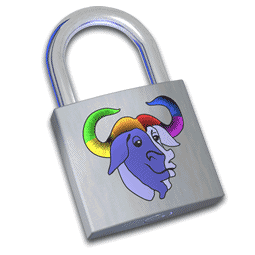
\includegraphics{images/gpg-logo.png}
%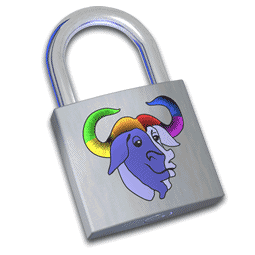
\includegraphics[scale=1]{images/gpg-logo.png}
\thispagestyle{empty}

%%\LARGE

%%\tableofcontents

\section{What is GPG?}

\textbf{GPG}, or GNU Privacy Guard is, in a nutshell, \textit{a free and easy way to send and receive emails completely securely}. The way most emails are currently sent is completely insecure, and is directly analogous to sending all of your mail on a postcard, available for any postman or eavesdropper along the way to read: we don't think this is good enough, and want to encourage more people to think and care about their privacy online.\\
\textbf{GPG} allows you to send \textbf{completely secure} emails to anyone else with an email address and a key: no special email provider is needed.

\section{How does it work?}
To make sure that only the intended recipient can read the email you've sent them, you need to encrypt the message. This means that to anyone without the right password (or `key') the message will look like random gibberish. \\As you may or may not have ever met the person you want to email, you probably won't have a way of agreeing a password without knowing for certain that no-one can intercept it (meaning they could read your messages too). Instead, as an analogy, you create an \textit{electronic padlock and key}, or \textbf{Public / Private Key Pair}. The Public Key is the padlock, and the Private Key is the key you use to unlock it. You mustn't send anyone a copy of the private key over the internet as someone could copy it, but instead you can send out an unlocked padlock (the public key) to anyone who wants to send you an email; this way they can `lock' (encrypt) the message with the padlock, but no-one, not even the sender can `unlock' (decrypt) it -- only you, the person with the private key can do that.\\ So that anyone can send you an email securely, you distribute your `open padlock' (Public Key) freely using a Key Server. Anyone can type in your name or email address and find your public key this way, but don't worry, there's no way anyone can work backwards from the Public Key to work out anything about your Private Key.

\section{Setup and usage guide}
\textit{(This is the \textbf{Mac} edition, so if you are using a different operating system please refer to CompSoc's GPG website, \href{http://gpg.compsoc.dur.ac.uk}{http://gpg.compsoc.dur.ac.uk}. Also go to the website for full screenshots of this walkthrough.)} 
\begin{compactenum}[1.]%itemize}
  \item Download and install the GPGTools software from \textbf{\href{http://www.gpgtools.org/}{http://www.gpgtools.org/}}
  \item Open `\textbf{GPG Keychain Access}' from the `Applications' folder - this is like Mac OS X's Keychain, but for Public / Private Keys. It will store your Public and Private Key Pair (in \textbf{bold}), and allow you to send emails to the people for whom you have public keys.
  \item On opening GPG Keychain Access for the first time, you'll be asked to generate a Public/Private Key Pair. Enter your name and email address, and then choose 'Advanced Options', specifying a Key Length of \textbf{4096} (this is a measure of how strong your key is). Leave everything else the same.
  \item Click 'Generate Key' and then when it starts working, bash away randomly at the keyboard for a minute or so: generating random data on the computer helps ensure that your key is as secure as possible.
  \item Think of and enter a secure passphrase - this isn't your Private Key, this is another layer of protection to ensure your Private Key remains secret, but it is still very important. Make sure the passphrase is at least 10 characters long. Enter it again for confirmation.
  \item You'll now see in the Keychain window a key with your name and email address in \textbf{bold}. You're all set to go! 
  \item Now you just need to look up keys for anyone you might want to talk to. Add `pgp.mit.edu' to the Keyserver field in `Preferences' (Cmd + ,), and then choose `Search for Key' (Cmd + F) to find someone else's public key. Try searching for `gpg@compsoc.dur.ac.uk' - that's us.
  \item Assuming you have your emails running in Mac Mail, open it up (from scratch) and you should now be able to send a test encrypted email to us. You should now see a locked padlock and a star with a tick in it below the subject line (right hand side) if you've entered the email address of someone you have a key for. Give it a try - send us an email!
  \item You'll have to enter your passphrase every time you send or receive an encrypted email - when you receive one, this is to unlock your private key to decrypt the message. When you send one, this is to unlock your private key to sign the email, to prove that it was you who sent it.
\end{compactenum}%itemize}
















\loggingall
\end{document}
\endinput
%%
%% End of file `leaflet-manual.tex'.
